\subsection{Råvaretabellen}
Efter afprøvning af prototyperne 2A og 2B på informanterne blev vi klar over at råvarer skal indtastes på forsiden i et design meget lig med Googles. Informanterne var glade for autocomplete-funktionen, der gør det muligt at indtaste teksten \textit{ba} i søge feltet og få stillet nogle forslag som \fx \textit{banan, balsamico}, så det ikke er nødvendigt at stave hele råvaren.
En autocomplete-funktion skal have noget data at stille forslag fra, og i dette tilfælde har vi brug for en tabel med alle de forskellige råvarer man kan forestille sig at en bruger vil indtaste. Denne tabel over råvarer vil fremover blive kaldt råvaretabellen.

Da opskrifterne, der søges på, kommer fra Arla, ville det have været nemt hvis Arla havde offentliggjort en liste over de forskellige ingredienser de benytter, således vi kunne bruge denne data som vores råvaretabel. En sådan liste var ikke til at finde, så vi begyndte at overveje muligheden for at lave råvaretabellen ved at udtrække ingredienserne direkte fra Arlas opskrifter. Et eksempel på ingrediensernes navne i Arlas opskrifter:

375 g rød peberfrugt i strimler

3 røde peberfrugter (ca. 600 g)

4 røde peberfrugter i store tern (ca. 500 g)

En bruger, der indtaster teksten \textit{pe} i forsøget på at indtaste \textit{rød peberfrugt}, skal kun præsenteres for forskellige råvarer, og altså ikke samme råvare i forskellige mængder og former (skiver, strimler, hakket, m.m.). Det vil sige, at de mange forskellige ingredienser, der alle består af en rød peberfrugt, kun skal medføre at \textit{rød peberfrugt} findes én gang i råvaretabellen. Vi vurderede at Arlas navngivning af ingredienser har været for forskellig til blive brugt som kilde til vores råvaretabel. Råvaretabellen er i stedet blevet lavet ud fra en liste af råvarer offentliggjort af madopskrifter. Et udpluk af listen ser således ud:

\begin{itemize}
\item Rød peberfrugt
\item Persille
\item Citron
\end{itemize}

Listen fra madopskrifter.nu blev brugt som vores råvaretabel af følgende grunde:

\begin{itemize}
\item Listen indeholdt kun 4 dubletter, som blev fjernet
\item Råvarerne indeholdt kun den rå råvare, ingen mængder eller andre betegnelser (vaskede, skrællede, m.m.)
\item Listen omfattede 933 råvarer, hvilket vi anså som rigeligt
\end{itemize}

Med en liste over råvarer, bliver det muligt for en bruger at indtaste en mængde råvarer. Udover dette har vi også brug for en mængde data, der fortæller noget omkring de opskrifter brugeren kan søge på. Denne data udtrækker vi fra Arlas hjemmeside, selvfølgelig med deres accept.

\section{Dataudtrækning}
For at kunne gemme informationer om en opskrifts forskellige bestanddele, såsom navn, tilberedningstid, m.m., er det nødvendigt at kunne udtrække denne data fra Arlas hjemmeside. Dette begreb kalder vi for dataudtrækning. Formålet er at indsætte data i databasen, så brugere har mulighed for at søge efter opskrifter, m.m. Da dataudtrækning kun har til formål at indsætte indhold i databasen, og ikke skal bestå af views eller controllers, har vi valgt at benytte Ruby uden Rails frameworket til dette. 
Opskrifterne på Arla blev udsat for dataudtrækning ved brug af modulet Nokogiri i Ruby. Nokogiri-modulet gør det let at finde værdier af forskellige elementer i et dokument. På Arlas hjemmeside findes en side, der giver mulighed for at vise alle opskrifterne. Der vises 16 opskrifter af gangen, og når man bladrer frem og tilbage imellem side 1 og side 2, hver især med 16 forskellige opskrifter på hver, så ændres en query i url'en på følgende måde: \\
\lstinline{?...\&paging=1\&...} \\
\lstinline{?...\&paging=2\&...} \\
En variabel ved navn \textit{paging} ændres i queryen værdi fra 1 til 2. Siderne, der indekserer 16 opskrifter af gangen er derfor lette at finde ved blot at lade en variablen \textit{paging} i queryen gå fra 1 og øges indtil ingen opskrifter fremkommer.

På hver enkelt indekseringsside vises 16 opskrifter. Et link til en opskrift på Arlas indekseringsside, ser i HTML således ud:

\lstinline{<h2><a href="/opskrifter/Suppe">Suppe</a></h2>}

Ved at bruge klassen \textit{xpath} i Nokogiri, kan alle 16 links hurtigt returneres som at array ved at benytte funktionen:

\texttt{xpath("//h2//a").map{|link| "http://www.arla.dk"+link["href"]}}

Metoden \textit{xpath}, leder efter alle \textit{<a>} tags inde i \textit{<h2>} tags og returnerer et array af elementer, der hver især har en værdi for indekset \textit{href}, der svarer til linket til siden. Ved at bruge funktionen \textit{map}, fås værdien af indekset \textit{href}, og præfixet \texttt{http://www.arla.dk} tilføjes foran. En forudsætning, der var til stede, for at kunne benytte denne metode, var at samme tagsekvens, i dette tilfælde \lstinline{<h2><a>}, ikke blev benyttet til andet end de links vi var interesserede i.

Med en mulighed for at finde alle opskrifters unikke url, begyndte vi at undersøge opbygningen af siden der viser en enkelt opskrift.
På samme måde kunne Nokogiri også bruges her til at finde informationer omkring tilberedningstid, opskriftens navn, billede af opskriften og portionsstørrelse. Alle disse ting kunne indsættes som en ny række i databasens tabel `recipes`. Opskriftens navn vær særlig nem at dataudtrække, da det var sidens titel, og kunne derfor tages fra HTML-tagget \textit{<title>}. Der var dog tilføjet lidt mere information, adskilt af karakteren ``|''. Et eksempel: \textit{Opskrifts navn | Kløver® | Produkter |}. Ved at bruge funktionen \textit{split} på karakteren ``|'', blev de forskellige dele, der var adskilt af ´´|'' hver især til ét element i et array. Opskriftens navn blev så det første element i arrayet.

Ingredienserne i en opskrift var nemme at dataudtrække på en lignende måde med Nokogiri, men hvordan de udtrukne ingredienser skulle håndteres var omfattende, og vil blive forklaret i \secref{sec:mapping}.

\subsection{Mapping af ingredienser}
\label{sec:mapping}
En råvaretabel i vores database, indeholder en liste over navnene på næsten 1000 råvarer. Denne liste giver brugeren mulighed for at indtaste en mængde råvarer i søgefeltet på {\Foodl}'s forside. Hvis han indtaster råvaren \textit{gulerødder}, skal han have muligheden for at udføre en søgning, der finder alle opskrifter, der indeholder gulerødder. Det er derfor nødvendigt for vores system at kunne oprette relationer imellem vores råvarer, og de opskrifter, der indeholder ingredienser magen til en råvare. Ingrediensernes navne i Arlas opskrifter er meget inkonsistente, og indeholder ofte også mængder, enheder, og forslag til Arlas egne produkter, der kan bruges. Derfor vil navnene på en ingrediens kun i få tilfælde svare til navnet på en råvare. Det er derfor nødvendigt med en metode til at finde den råvare, som en ingrediens \textit{minder} mest om. Denne proces vil vi fremover kalde for mapping. For at kunne finde ud af hvilken råvare, en give ingrediens minder mest om, er det nødvendigt med at godt grundlag at sammenligne på. En ingrediens bør derfor analyseres på en måde, så mængde, enhed og andre ting, der er ligegyldige for sammenligningen, udelades. Metoden til dette vil blive kaldt for \methodref{IngredientAnalyzer}. Dernæst er det også nødvendigt med en metode, der kan sammenligne to strenge og afgøre, hvor meget de minder om hinanden. Denne metode, vil vi fremover kalde \methodref{CompareStrings}.

\subsubsection{Optimering}
Hvis \methodref{CompareStrings} køres hver gang der udføres en søgning, vil det stille høje krav til hastigheden af denne funktion, for at brugeren kan udføre en hurtig søgning. For ikke at sætte krav til hastigheden af funktionen, benyttede vi en relationstabel. For hver opskrift fundet på Arla sammenlignede vi hver enkelt ingrediens i opskriften med alle råvarerne i råvaretabellen ved at bruge funktionen \methodref{CompareStrings}. For hver ingrediens blev én relation indsat mellem ingrediensen og den råvare i råvaretabellen, som ingrediensen bedst matcher ifølge vores \methodref{CompareStrings}. Når en bruger udfører en søgning, vil \methodref{CompareStrings} slet ikke blive benyttet. Det vil kun være nødvendigt at undersøge de indtastede råvares relationer til ingredienser, og blot præsentere de opskrifter, der er relateret til de fundne ingredienser, som et søgeresultat for brugeren.

\subsubsection{IngredientAnalyzer}
Inden en ingrediens sammenlignes med en råvare, så er det nødvendigt at foretage en analyse af ingrediensen. Ingredienserne på Arlas opskrifter består nemlig af både navn, mængde og enhed, mens indholdet i vores råvaretabel kun består af en råvares navn. Første skridt i behandlingen af de udtrukne ingredienser fra Arlas opskrifter, var at fjerne mængder og enheder. Dette fik klassen \classref{IngredientAnalyzer} ansvaret for. Arla var meget konsistente i deres syntaks, hvad angik mængde og enhed. Syntaksen var altid: \textbf{``mængde enhed navn''}.
På den måde kunne vi nemt udtrække en ingrediens' mængde, enhed og navn, ved at lade \classref{IngredientAnalyzer} starte ved første karakter. Hvis denne er en numerisk karakter, fortsættes der, indtil et mellemrum, og den fundne streng blev bestemt som ingrediensens mængde. Dernæst tjekkes om den resterende streng starter med en enhed, som \fx \textit{dl, kg, bundt, glas} efterfulgt af et mellemrum. Vi havde gemt en liste over alle, af Arla benyttede, mængder. Hvis en enhed kunne identificeres, blev denne bestemt til at være ingrediensens enhed. Den resterende streng blev bestemt til at være ingrediensens navn.
Nogle specielle ingredienser var uden mængde og enhed, \fx \textit{vand}, men fordi en sådan ingrediens ikke starter med en numerisk karakter, springes mængden over. Enheden springes også over, da \textit{vand} ikke findes på listen over enheder, og for den sags skyld heller ikke ender med et mellemrum. Derfor vil ingrediensens navn stadig blive bestemt til at være \textit{vand}, uden en mængde og enhed.

\subsubsection{TextComparer}
Der findes mange forskellige algoritmer til at sammenligne to strenge for lighed. Det er vigtigt for os at finde en god og brugbar metode, der så korrekt som muligt kan mappe alle ingredienserne i Arlas opskrifter over til en passende råvare i vores råvaretabel. Dette ansvar blev lagt på klassen \classref{TextComparer} med metoden \methodref{CompareStrings}. Det har ikke været muligt for os at opnå en 100 \% korrekt mapping ved brug af en algoritme til dette, og vi har derfor også foretaget en stor del af mappingen manuelt. Vi har erfaret, at der ved brug af en algoritme nemt kan opstå problemer omkring ingredienser der minder meget om hinanden, som \fx ved mapping af ingrediensen \textit{hakket løg}. En algoritme vil have svært ved at vide, at \textit{hakket løg} skal mappes til råvaren \textit{løg} og ikke \textit{hakket oksekød}. En korrekt mapping vil i dette tilfælde kræve kendskab til at ordet \textit{hakket} er et udsagnsord og derfor bør fjernes før der forsøges at mappe. Men hvis vi vil mappe ingrediensen \textit{hakket oksekød}, så er det nødvendigt at ordet \textit{hakket} stadig indgår under mappingen (på trods af at det er et udsagnsord), fordi der findes mange former for oksekød og vi ønsker at skelne imellem de forskellige former.

Efter at dataudtrækkeren har fundet en ingrediens' navn, skal det undersøges hvilken råvare fra vores råvaretabel, denne minder mest om. De er begge to strenge, så der vil være brug for en metode til at sammenligne hvor ens to strenge er, og derved finde ud af hvilken streng i råvaretabellen, der minder mest om ingrediensens navn.
Vi har brugt tilfældigt udvalgte ingredienser fra Arlas opskrifter til at teste 5 forskellige metoder til tekstsammenligning. I mange tilfælde kunne alle 5 metoder mappe en ingrediens til en korrekt råvare. I enkelte tilfælde skete der dog en fejlmapping, og disse fejlmappings brugte vi til at sammenligne hvilken metode, der lavede færrest fejl. Resultatet kan ses i \tableref{table:test-af-compares}.

\paragraph{Forklaring af de forskellige \methodref{CompareStrings} funktioner}
\begin{enumerate}
\item Egen algoritme (lineær)
\item Egen algoritme (polynomial)
\item Levenshtein (1 point for slet, tilføj og udskift) %kilde ruby gem levenshtein.distance
\item Levenshtein (1 point for slet, tilføj og udskift. Score divideres med længste streng) %kilde ruby gem levenshtein.normalized_distance
\item Levenshtein (1 point for slet og tilføj. 2 point for udskift) %kilde ruby gem text.levenshtein.distance med modificeret vægt
\end{enumerate}


\begin{table}
    \begin{tabular}{|p{2cm}|c|c|c|c|c|}
        \hline
        Ingrediens                                                 & Metode 1        & Metode 2                & Metode 3           & Metode 4           & Metode 5        \\ \hline
        dildkvist                                                  & \textbf{dild}            & \textbf{dild}                    & \textbf{dild}               & sildefilet         & dild            \\ \hline
        groft salt                                                 & \textbf{salt}            & citron saft             & frugtsaft          & frugtsaft          & \textbf{salt}            \\ \hline
        grofthakkede krydderurter, fx koriander, persille og dild & \textbf{krydderurtemix}  & \textbf{tikka (indisk krydderi)} & hakkede tomater    & hakkede tomater    & hakkede tomater \\ \hline
        basmatiris eller luftige urteris                           & \textbf{basmati ris}     & herbamare urtebouillon  & \textbf{basmati ris}        & \textbf{basmati ris}        & \textbf{basmati ris}     \\ \hline
        ostindisk karry                                            & \textbf{karrypasta}      & kinaradise              & sød sherry         & sød sherry         & \textbf{karry}           \\ \hline
        frisk salvie                                               & \textbf{salvie}          & \textbf{salvie}                  & fiskesauce         & fiskesauce         & \textbf{salvie}          \\ \hline
        koncentreret tomatpure                                     & \textbf{tomatpure}       & \textbf{tomatpure}               & soltørrede tomater & soltørrede tomater & \textbf{tomatpure}       \\ \hline
        hakket svinelever                                          & hakket svinekød & \textbf{svinelever}              & hakket svinekød    & hakket svinekød    & \textbf{svinelever}      \\ \hline
        store kapers med stilk                                     & \textbf{kapers}          & syltede artiskokhjerter & trefarvet is       & trefarvet is       & \textbf{kapers}          \\ \hline
        hvidvin fx rieslin                                         & \textbf{hvidvin}         & \textbf{hvidvin}                 & hvidvinseddike     & hvidvinseddike     & \textbf{hvidvin}         \\ \hline
        friskpresset limesaft                                      & \textbf{limesaft}        & \textbf{limesaft}                & appelsinsaft       & appelsinsaft       & \textbf{limesaft}        \\ \hline
        kartoffel                                                  & \textbf{kartofler}       & \textbf{kartofler}               & \textbf{kartofler}          & \textbf{kartofler}          & kartoffelmel    \\ \hline
        ~                                                          & ~               & ~                       & ~                  & ~                  & ~               \\ \hline
        Total:                                                     & 11              & 7                       & 3                  & 2                  & 10              \\
        \hline
    \end{tabular}
  \caption{Test af flere forskellige \methodref{CompareStrings} funktioner, der bruges til at mappe en ingrediens til en råvare. Fed skrift betyder at begge vores informanter har godkendt mappingen. Se \apref{ap:valgafmappingmetode}}  \label{table:test-af-compares}
\end{table}

Som det ses i \tableref{table:test-af-compares}, var metode 1 den, der gav den bedste mapping. Metoden fik 11 rigtige ud af 12 mulige, men det bør bemærkes at sammenligningen kun er foretaget på de ingredienser, som mindst én metode mappede forkert. Vi kom forbi 56 ingredienser udover de ingredienser vist i tabellen, før vi tilsammen havde 12 ingredienser, som én eller flere metoder mappede forkert. 

Metode 1 er en algoritme vi selv har udviklet, der er beskrevet med pseudokode i \pseudoref{alg:compare}. Den tager to strenge som input, og returnerer en værdi mellem 0 og 100. Højere returværdi betyder større lighed mellem de to inputtede strenge. 100 point opnås kun ved to identiske strenge. Idéen bag algoritmen er, at to inputtede strenge, $a$ og $b$ hele tiden sammenlignes for at finde den længste streng de har til fælles. Denne streng fjernes fra $a$ og $b$, og en score med længden af fællesstrengen i anden potens. Sådan fortsættes indtil $a$ og $b$ ikke længere har nogen streng til fælles. Dette er også tilfældet, hvis én eller begge er tomme strenge. Ligheden mellem de to strenge beregnes ved at finde ud af hvor stor en procentdel den endelige score udgør af den maksimalt opnåelige score, der fås kun hvis $a = b$.
I \tableref{table:vores-compare-eksempel} ses et eksempel på hvordan algoritmen sammenligner \textit{hummersuppe} med \textit{suppe med hummerhale} og kommer frem til resultatet $13.8$.

\begin{table}
    \begin{tabular}{|l|l|l|}
        \hline
        str1        & str2                  & ~                             \\ \hline
hummersuppe & suppe med hummerhaler & $max\_length = 21$               \\         
        \textbf{hummer}suppe & suppe med \textbf{hummer}haler & $score = 6^2 = 36$               \\ 
        \textbf{suppe}       & \textbf{suppe} med haler       & $score = score + 5^2 = 36 + 25 = 61$                 \\ 
        ~           &  med haler            & $no common substrings found$        \\ 
        ~           & ~                     & $max\_score = 21^2  = 441$    \\ 
        ~           & ~                     & $return \frac{61 \times 100}{441} = 13.8$ \\
        \hline
    \end{tabular}
    \caption{Her vises et eksempel på hvordan vores algoritme sammenligner \textit{hummersuppe} med \textit{suppe med hummerhaler}.}
    \label{table:vores-compare-eksempel}
\end{table}

Metode 2 var magen til metode 1, bortset fra at scoren kun blev forøget med længden af den fælles streng, og ikke i anden potens som i metode 1 (se \pseudoref{alg:compare}, linje 7). På samme måde blev variablen $max\_score$ i linje 5 også beregnet lineært.

\begin{algorithm} [H]
	\capt{Algoritmen udregner hvor ens to strenge er.}
	\label{alg:compare}
	\begin{algorithmic}[1]
\Function{CompareStrings}{str1, str2}

\State $max\_size \gets \max(str1.length, str2.length)$
\If{$max\_size == 0$}
	\State return $100$
\EndIf
\State $score \gets 0$

\While{a longest substring $ls$ exists in both $str1$ and $str2$}
	\State $score \gets score + ls.length^2 $
	\State remove $ls$ from $str1$ and $str2$
\EndWhile

\State $max\_score \gets \max\_size^2$
\State $return \frac{score}{max\_score * 100} $

\EndFunction
\end{algorithmic}
\end{algorithm}

\begin{algorithm} [H]
	\capt{Algoritmen finder den længste fælles streng, som er indeholdt i begge de strenge, der gives som input.}
	\label{alg:longest-common-substring}
	\begin{algorithmic}[1]
\Function{LongestCommonSubstring}{$a = \{a_0, a_1, ... , a_n\}, b = \{b_0, b_1, ... , b_m\}$}
\State $max\_length \gets 0$
\For{$x = 0 \to n$}
  \For{$y = 0 \to m$}
    \State $count[x, y] \gets 1$
    \If{$x > 0 \wedge y > 0$}
      \State $count[x, y] \gets count[x, y] + count [x-1, y-1]$
    \EndIf
    \If{$count[x, y] > max\_length$}
      \State $max\_length \gets count[x, y]$
      \State $end\_pos \gets x$
    \EndIf
    \State $start = end\_pos - max\_length - 1$
    \State \Return $\{a_{start}, a_{start+1}, ... , a_{end\_pos}\}$
  \EndFor
\EndFor
\EndFunction
\end{algorithmic}

\end{algorithm}

\pseudoref{alg:longest-common-substring} er en pseudokode vi selv har skrevet, for at beskrive en ruby-implementation\cite{longestcommonsubstringrubywiki} af funktionen \methodref{LongestCommonSubstring}. \methodref{LongestCommonSubstring} er en algoritme, der har til formål, blandt to strenge, at finde den længste streng, som disse to har til fælles. Eksempel: \methodref{LongestCommonSubstring(\textit{``ostemad''}, \textit{``olivensten''}) = ``ste'')}. Et eksempel på hvordan algoritmen beregner den længste fælles streng blandt \textit{smørremad} og \textit{ørred} til at være \textit{ørre}, kan ses i \figref{fig:longest-common-substring}.
Algoritmen laver et 2-dimensionelt array af størrelsen $n \times m$, hvor $n$ og $m$ er længden af de inputtede strenge $a$ og $b$. Hver karakter i $a$ og $b$ sammenlignes i læseretningen af arrayet, se \figref{fig:longest-common-substring}. Hvis karakten $a_x$ er ikke er lig med $b_y$, så indsættes værdien 0 i arrayet. Er de ens, så indsættes værdien $1 + [a_{x-1}, b_{y-1}]$.
Variablen $max\_length$ indeholder altid den største værdi i arrayet, mens $end\_pos$ holder den værdi $x$ havde, da $max\_length$ sidst blev assignet til.
Når algoritmen er færdig, er $end\_pos$ i dette tilfælde lig med 5, hvor begge strenge har karakteren \textit{e}. $max\_length$ er 4, så ved at gå 3 karakterer tilbage fra $end\_pos$ fås de 4 karakterer \textit{ørre}, som returneres i linje 14. Kompleksiteten af denne funktion beregnes ved at betragte løkken på linje 3, der eksekveres $n$ gange, hvori løkken på linje 4 er indeholdt, der eksekveres $m$ gange. Alle operationer inden i løkken på linje 4's scope kan udføres i konstant hastighed, hvilket betyder at algoritmens kompleksitet er $O(n \times m)$.

Funktionen \methodref{CompareStrings}, der kalder funktionen \methodref{LongestCommonSubstring} kan nu beregnes ved at betragte løkken på linje 7 i \methodref{CompareStrings}. For hver iteration af løkken, fjernes minimum én karakter fra begge de strenge, der sammenlignes. Hvis én af de to strenge er tomme, trædes der ud af løkken. Derfor vil løkken maskimalt blive itereteret $n$ gange, hvor $n$ er længden af den korteste af de to inputtede strenge.
Da hver iteration af løkken kalder \methodref{LongestCommonSubstring} én gang, hvis kompleksitet er $O(n \times m)$, bliver \methodref{CompareStrings} kompleksitet $O(n^2 \times m)$. Hvis inputtet er strenge af samme længde, er kompleksiteten $O(n^3)$.
\begin{figure}
\centering
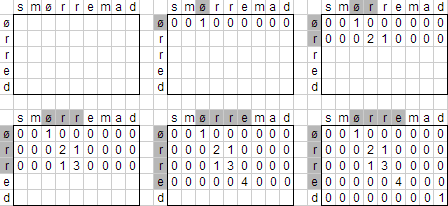
\includegraphics[scale=1]{billeder/longest-common-substring.png}
  \capt{Et eksempel på hvordan funktionen longest\_common\_substring virker.}
  \label{fig:longest-common-substring}
\end{figure}

\subsubsection{Mapping af ingredienser til råvarer}
Den automatiske mapping omfattede 10,234 ingredienser, blandt 921 opskrifter. Tidsforbruget var ca. 4 timer, og langt de fleste ingredienser blev mappet korrekt. Ind i mellem gik mappingen galt, fx. blev ingrediensen \textit{groftkværnet peber} hver gang mappet til råvaren \textit{hvid peber} i stedet for råvaren \textit{peber}. For at få en bedst muligt mapping besluttede vi os for at gå alle mappings igennem igennem manuelt. Under mappingen havde vi gemt returværdien af \methodref{CompareStrings(string, string)}, der fortæller hvor ens de to sammenlignede tekstrenge var. Ved at have gemt returværdien behøver vi ikke at kontrollere mappings, der har returneret 100, da det vil sige at ingrediensen er blevet mappet til en identisk råvare. På denne måde kunne vi se bort fra 1,236 ingredienser, der ikke behøvede manuel kontrol.
Til at mappe ingredienserne hurtigst muligt lavede vi et meget simpelt WinForms program med Visual Studio, skrevet i C\# (se \apref{ap:manuel-mapping}). Programmet gjorde det muligt at få vist 20 labels med ingredienser. Ud for hvert label blev vist et tekstfelt med den råvare, som ingrediensen var blevet mappet til. Ved at ændre i tekstfeltet kunne man hurtigt få lavet en korrekt mapping. Vi tilføjede flere funktionaliteter for at øge hastigheden vi kunne mappe med.
\begin{itemize}
\item Ingredienserne blev sorteret alfabetisk. Omkring 120 ingredienser i træk var \textit{grofthakket peber}.
\item Autocomplete gjorde det nemt at se hvilke råvarer man kunne vælge imellem og også hurtigere at indtaste råvaren.
\item Råvarer kunne tilføjes hvis ingen fandtes, der matchede en given ingrediens.
\item Ingredienser som \fx \textit{grillspyd} og \textit{lagkageflag} kunne fjernes i programmet.
\item En hel side kunne godkendes med ét klik, hvis alt var mappet korrekt på forhånd.
\end{itemize}

Tidsforbruget på remappingen var ca. 6 mandetimer, hvilket kan omregnes til $\frac{10234 - 1236}{6} = 1500$ ingredienser pr. mandetime.
